\par\noindent\begin{minipage}{\linewidth}
% !TeX root = ../教材题库_全部条目_转写工作稿.tex
% Source: XJ-B1-C01-RV-P029-Y1165
% 第1章 / 章末复习 复习题一 / 教材 p.29 / PDF 第36页
% 已对照原页转写题干及公式；待教师复核；未制作答案
% 原题及相邻原解截图（核对用）：../题目原图/XJ-B1-C01-RV-P029-Y1165-01.webp
% 本文件只在转写完成后作为题干使用；OCR 条目尚不是可靠题干。
\begin{bankitem}{复习题一 第7题}{第1章 / 章末复习 复习题一 / 教材 p.29 / PDF 第36页}{XJ-B1-C01-RV-P029-Y1165}{已对照原页转写题干及公式；待教师复核；未制作答案}
已知全集为 $U$，集合 $A,B,C$ 都是 $U$ 的子集，用集合 $U,A,B,C$ 表示图中的阴影部分。
\begin{center}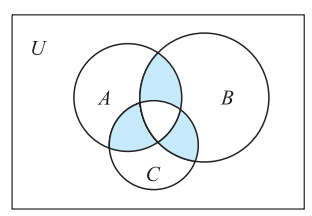
\includegraphics[width=6cm]{figures/C01-RV07.png}\end{center}
\end{bankitem}
\end{minipage}\par\medskip
